\documentclass[11pt,twocolumn,letterpaper]{article}

\usepackage{cvpr}
\usepackage{times}
\usepackage{epsfig}
\usepackage{graphicx}
\usepackage{amsmath}
\usepackage{amssymb}
\usepackage{CJKutf8}
\usepackage{graphicx} %插入图片的宏包
\usepackage{float} %设置图片浮动位置的宏包
\usepackage{subfigure} %插入多图时用子图显示的宏包

% Include other packages here, before hyperref.

% If you comment hyperref and then uncomment it, you should delete
% egpaper.aux before re-running latex.  (Or just hit 'q' on the first latex
% run, let it finish, and you should be clear).
\usepackage[breaklinks=true,bookmarks=false]{hyperref}

\cvprfinalcopy % *** Uncomment this line for the final submission

\def\cvprPaperID{****} % *** Enter the CVPR Paper ID here
\def\httilde{\mbox{\tt\raisebox{-.5ex}{\symbol{126}}}}

% Pages are numbered in submission mode, and unnumbered in camera-ready
%\ifcvprfinal\pagestyle{empty}\fi
\setcounter{page}{1}
\begin{document}
\begin{CJK*}{UTF8}{bsmi}

%%%%%%%%% TITLE
\title{DEEP CONVOLUTION NEURAL NETWORK FOR DETECTION OF FAULTY SOLAR PANELS}

\author{Team member: 顏領呈\\
學號: Q36081575\\
{\tt\small darkness851106@gmail.com}
% For a paper whose authors are all at the same institution,
% omit the following lines up until the closing ``}''.
% Additional authors and addresses can be added with ``\and'',
% just like the second author.
% To save space, use either the email address or home page, not both
}

\maketitle
%\thispagestyle{empty}

%%%%%%%%% BODY TEXT
\section{Introduction}
Due to the fossil fuel is exhausted and causing problem, such as air pollution, acid rain, soil pollution, and so on. Now, many countries are interested in the new and reusable energy and want to minimize the damage caused by the use of fossil fuels. It results in interesting of the new and renewable energy. Therefore, solar photovoltaic energy production as a new and reusable energy, which becomes more and more important in this world. As the use of solar photovoltaic energy grows, more efficient ways are needed to build, operate, and maintain the solar industry.

The solar panel is greatly affected by the outdoor environment, such as the dust attached to the panel, sun hiding in the clouds, and etc. This requires some maintenance work for the user. {\bf However, there are a lot of problems that the user cannot just judge by their eyes. Such as fault of solar panel, disconnection of the panel itself and hard to see what is attached to the solar panel.} Therefore, the automatic detecting faulty solar panel system is essential. 

In this project, {\bf I propose a detecting system of faulty solar panel using drones, and thermal cameras.} However, I focus on the processing of the image, which means that I do not need to know how to let drones take pictures of solar panels. 

In order to detect the image faulty more easily, I need to get thermal image. Hence, the error of the photovoltaic panel is determined using the thermal imaging camera by drones. Once I get the picture, I will start to analyze the problem of solar panels, and then I report the problem to help for maintenance of solar panels.
%------------------------------------------------------------------------
\section{System framework}
This section talks about what I'm going to do in the experiment. First, I get the thermal image of solar panels from drones, and then I convert the RGB image to grayscale. Second, I find boundary of image by "Canny edge detection algorithm". If the boundary of image is rectangle, I go to next step, else I start over to get a new thermal image from drones. Third, in order to decide how many times I need to detect the solar panels, I count the number of solar panels in the image. Fourth, I draw rectangle boundary and find solar panel array. Fifth, I start to detect the problem for each solar panel. Sixth, I get information of solar panel. If there is faulty, I go to next step(because I detect the problem, then I can go to detect next solar panel), else I start over to get next solar panel. And keep doing this until the number of solar panel is zero. 



%-------------------------------------------------------------------------
\subsection{Flow chart}
\begin{figure}[H] %H为当前位置,!htb为忽略美学标准,htbp为浮动图形
\centering %图片居中
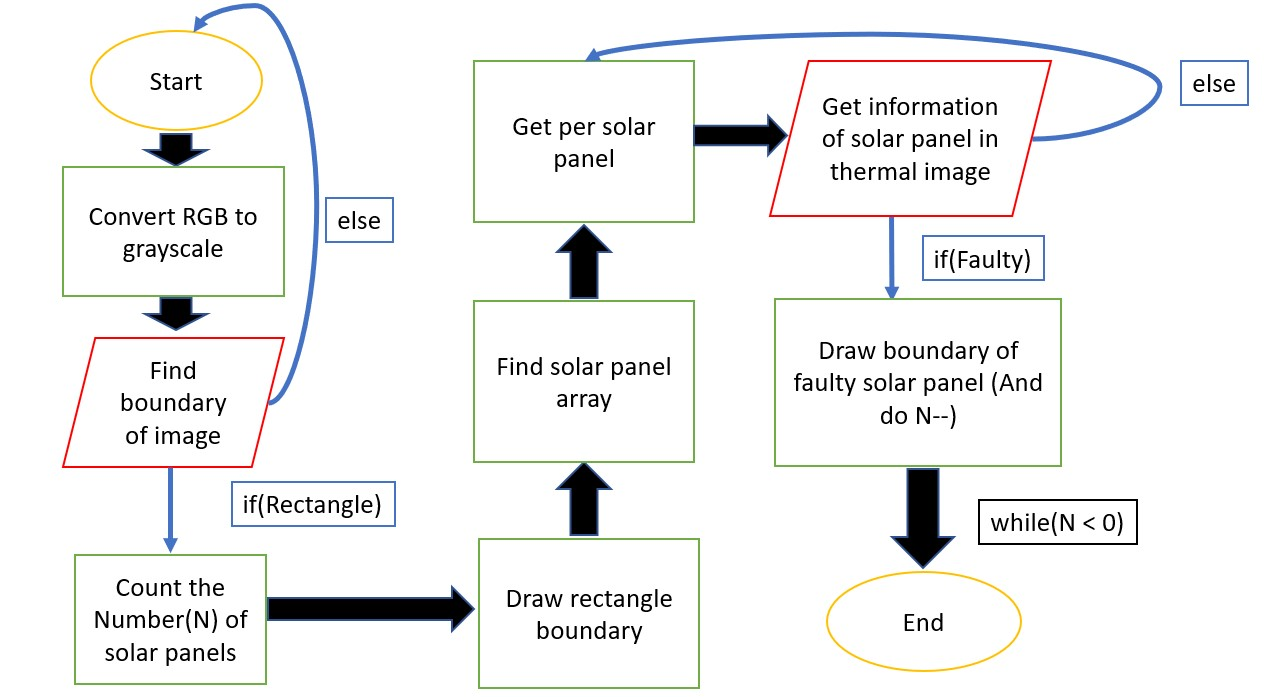
\includegraphics[width=0.56\textwidth]{flowchart.jpg} %插入图片,[]中设置图片大小,{}中是图片文件名
\caption{Experimental design} %最终文档中希望显示的图片标题
\label{Fig.main2} %用于文内引用的标签
\end{figure}


%-------------------------------------------------------------------------
\subsection{Tools and environments}
Canny Edge Detection Algorithm: To get the edge of the thermal image so that I can find boundary of the solar panel.

OpenCV Blob Detection: To get the blob of solar panel so that I can detect the problem.



%------------------------------------------------------------------------
\section{Expected results}
I can successfully detect the problem of the solar panel. Also, I can classify and analyze the problem of the solar panel, such as “Cell”, “Cracking”, “Shadowing”, “Soiling” and etc. “Cell” means that hot spot occurring with square geometry in single cell. “Cracking” means that module anomaly is caused by cracking on module surface. “Shadowing” means that sunlight is obstructed by vegetation, man-made structures, or adjacent rows. “Soiling” means that dirt, dust, or other debris are on surface of module.

%------------------------------------------------------------------------
\subsection{Dataset description}
The dataset consists of 200 infrared images that are 750 by 840 pixels each. There are 12 defined classes of solar modules presented in this project with 11 classes of different anomalies and the remaining class being No-Anomaly (i.e. the null case).


%------------------------------------------------------------------------
\begin{thebibliography}{99}  
\bibitem{ref1}XIAOJIN GONG, QI YAO, MENGLIN WANG, AND YING LIN, “A Deep Learning Approach for Oriented Electrical Equipment Detection in Thermal Images”, Received June 7, 2018, accepted July 11, 2018, date of publication July 23, 2018, date of current version August 20, 2018.  
\bibitem{ref2}MANISH BHATTARAI, AND MANEL MARTÍNEZ-RAMÓN, “A Deep Learning Framework for Detection of Targets in Thermal Images to Improve Firefighting”, Received February 13, 2020, accepted May 5, 2020, date of publication May 11, 2020, date of current version May 21, 2020.  
\bibitem{ref3}Chih-Hsueh Lin, Zhi-Hao Wang , and Gwo-Jia Jong, “A De-Identification Face Recognition Using
Extracted Thermal Features Based on Deep Learning”, IEEE SENSORS JOURNAL, VOL. 20, NO. 16, AUGUST 15, 2020.
\bibitem{ref4}ROSLIDAR ROSLIDAR, AULIA RAHMAN, RUSDHA MUHARAR, MUHAMMAD RIZKY SYAHPUTRA, “A Review on Recent Progress in Thermal Imaging and Deep Learning Approaches for Breast Cancer Detection”, Received May 21, 2020, accepted June 14, 2020, date of publication June 22, 2020, date of current version July 2, 2020.
\bibitem{ref5}Cai Lile, Li Yiqun, “ANOMALY DETECTION IN THERMAL IMAGES USING DEEP NEURAL NETWORKS”, Institute for Infocomm Research, Singapore.  
\bibitem{ref6}Vijay Paidi, Hasan Fleyeh, Roger G. Nyberg, “Deep learning-based vehicle occupancy detection in an open parking lot using thermal camera”, IET Intelligent Transport Systems.  
\bibitem{ref7}Miguel Bordallo Lopez, Carlos R. del-Blanco, Narciso Garcia, “Detecting exercise-induced fatigue using thermal imaging and deep learning”, Center for Machine Vision and Signal Analysis, University of Oulu, Finland.  
\bibitem{ref8}SungWon Lee, Kwang Eun An, Byung Don Jeon, Kyoung Yeon Cho, Seung Jae Lee, “Detecting Faulty Solar Panels Based on Thermal Image Processing”, School of Information Technology Engineering, Catholic University of Daegu, Republic of Korea.  
\bibitem{ref9}Yuan-Tsung Chen, Ming-Shi Wang, “Human Face Recognition Using Thermal Image”, Received 2 May 2002; Accepted 12 June 2002.
\bibitem{ref10}G. A. Licciardi, and J. Chanussot, “Nonlinear PCA for Visible and Thermal Hyperspectral Images Quality Enhancement”, IEEE GEOSCIENCE AND REMOTE SENSING LETTERS, VOL. 12, NO. 6, JUNE 2015. 
\bibitem{ref11}Zhan Wu, Min Peng, Tong Chen, “Thermal Face Recognition Using Convolutional Neural Network”, 2016 International Conference on Optoelectronics and Image Processing. 
\end{thebibliography}

\end{CJK*}
\end{document}
